%-------------------------------------------------------------------------------------------------%
% Author: John Joseph Valletta
% Date: 18/02/2015
% Title: Clustering
%-------------------------------------------------------------------------------------------------%
% Preamble
\documentclass[pdf]{beamer}
\usepackage{textpos} % for logo placement in headline
\usepackage[export]{adjustbox}
%-------------------------------------------------------------------------------------------------%
\usepackage{listings} % To insert code
\usepackage{color}
\definecolor{dkgreen}{rgb}{0,0.6,0}
\definecolor{gray}{rgb}{0.5,0.5,0.5}
\definecolor{mauve}{rgb}{0.58,0,0.82}
\definecolor{deepblue}{rgb}{0,0,0.5}
\definecolor{deepred}{rgb}{0.6,0,0}
\definecolor{deepgreen}{rgb}{0,0.5,0}
\definecolor{lightgray}{rgb}{0.90,0.90,0.90}
\lstdefinestyle{RCode}{
language=R,                     % the language of the code
basicstyle=\scriptsize\ttfamily,       % the size of the fonts that are used for the code
numbers=none,%left,                   % where to put the line-numbers
numberstyle=\tiny\color{gray},  % the style that is used for the line-numbers
stepnumber=1,                   % the step between two line-numbers. If it's 1, each line
                          % will be numbered
numbersep=5pt,                  % how far the line-numbers are from the code
backgroundcolor=\color{lightgray},  % choose the background color. You must add \usepackage{color}
showspaces=false,               % show spaces adding particular underscores
showstringspaces=false,         % underline spaces within strings
showtabs=false,                 % show tabs within strings adding particular underscores
frame=lines,%single,                   % adds a frame around the code
rulecolor=\color{black},        % if not set, the frame-color may be changed on line-breaks within not-black text (e.g. commens (green here))
tabsize=2,                      % sets default tabsize to 2 spaces
captionpos=b,                   % sets the caption-position to bottom
breaklines=true,                % sets automatic line breaking
breakatwhitespace=false,        % sets if automatic breaks should only happen at whitespace
title=\lstname,                 % show the filename of files included with \lstinputlisting;
                          % also try caption instead of title
keywordstyle=\color{blue},      % keyword style
commentstyle=\color{dkgreen},   % comment style
stringstyle=\color{mauve},      % string literal style
escapeinside={\%*}{*)},         % if you want to add a comment within your code
morekeywords={}            % if you want to add more keywords to the set
}
%-------------------------------------------------------------------------------------------------%
\newif\ifplacelogo % Create a new conditional to avoid displaying logo on every slide
\placelogotrue % Set it to true
\mode<presentation>{\usetheme{Madrid}} % default Antibes Berlin Madrid Montpelier Ilmenau CambridgeUS Berkeley Singapore Copenhagen Malmoe Warsaw
\usecolortheme{dolphin}
\useinnertheme{circles} % circles, rectanges, rounded, inmargin
\usefonttheme[onlymath]{serif} % Makes math fonts like the usual LaTeX ones
%\useoutertheme{tree} % infolines, smoothbars, sidebar, split, tree
\setbeamercovered{transparent=5} % Transparent 10% overlays
\setbeamertemplate{caption}{\raggedright\insertcaption\par} % Remove the word "Figure" from caption %\setbeamertemplate{caption}[default]
\setbeamertemplate{navigation symbols}{} % don't put navigation tools at the bottom (alternatively \beamertemplatenavigationsymbolsempty)
\graphicspath{ {./Figures/} }

% Titlepage
\title{Clustering}
\subtitle{(unsupervised learning)}
\author{John Joseph Valletta}
\date[1st-2nd June 2015]{1st-2nd June 2015}
\institute[]{University of Exeter, Penryn Campus, UK}
% \logo{
%   \makebox[0.95\paperwidth]{
%     
\includegraphics[width=4cm,keepaspectratio]{logo1.pdf}
%     \hfill
%     
\includegraphics[width=4cm,keepaspectratio]{logo2.pdf}
%   }
% }
% Logo
\logo{\ifplacelogo
\includegraphics[width=4cm,keepaspectratio, left]{logo2.pdf}\fi}
\addtobeamertemplate{headline}{}{\ifplacelogo
\begin{textblock*}{100mm}(.68\textwidth,+0.1cm)%.015 instead of 0.68 originally

\includegraphics[width=4cm,keepaspectratio]{logo1.pdf}
\end{textblock*}\fi}

%-------------------------------------------------------------------------------------------------%
% Start of Document
%-------------------------------------------------------------------------------------------------%
\begin{document}
%-------------------------------------------------------------------------------------------------%
% Slide 0: Title Slide
\begin{frame}
\titlepage
\end{frame}
\placelogofalse % Turn logo off
%-------------------------------------------------------------------------------------------------%
\begin{frame}{Overview}
\begin{itemize}\addtolength{\itemsep}{0.5\baselineskip}
	\item<2-> What is clustering?
	\item<3-> Major types of clustering methods
	\item<4-> $k$-means clustering
	\item<5-> Agglomerative hierarchical clustering
	\item<6-> Gaussian mixture models
	\item<7-> How do we determine the correct number of clusters?
\end{itemize}
\end{frame}
%-------------------------------------------------------------------------------------------------%
\begin{frame}{What's the problem?}
Well, it's driven by your data, e.g which of these genes are co-regulated?
\begin{center}
	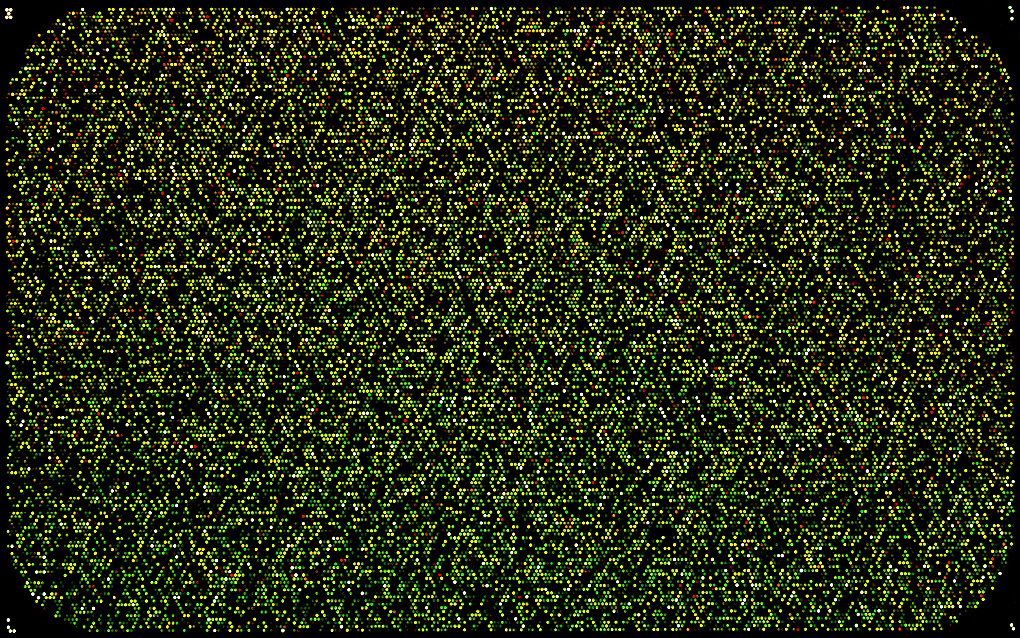
\includegraphics[width=0.8\textwidth]{microArray.jpg}
\end{center}
We want to find some underlying structure in the data $\rightarrow$ \textbf{Clustering}
\end{frame}
%-------------------------------------------------------------------------------------------------%
\begin{frame}{What's the problem?}
\begin{description}[Mathematical chemistry:]\addtolength{\itemsep}{0.5\baselineskip}
	\item [Gene expression:] discovering co-regulated genes
	\item [Biological systematics:] finding organisms sharing similar attributes
	\item [Computer vision:] segmenting a digital image for object recognition
	\item [Epidemiology:] identifying geographical clusters of diseases  
	\item [Medical imaging:] differentiating between tissues
	\item [Mathematical chemistry:] grouping compounds by topological indices
\end{description}
\vfill
\textbf{Clustering is particularly useful in applications where labelling the data is very time consuming/expensive} 
% Mention that it's also used in market research, social network analysis, search engines Clusty etc...
\end{frame}
%-------------------------------------------------------------------------------------------------%
\begin{frame}{What is clustering?}
\visible<1->{\begin{block}{Formal definition}
Identifying homogeneous and well separated groups of data points (features) by some similarity
measure
\end{block}}
\vfill
\visible<2->{\begin{block}{Informal definition}
The process of stereotyping your data \\
e.g \textit{these} are round(ish) faces, \textit{these} are short(ish) people
\end{block}}
\vfill
\visible<3->{\begin{block}{But how many groups?}
An unsolved problem. Issue lies in the subjectivity of the word \textbf{\textit{similar}} and its
mathematical definition
\end{block}}
\end{frame}
%-------------------------------------------------------------------------------------------------%
\begin{frame}{Are they similar?}
\begin{center}
	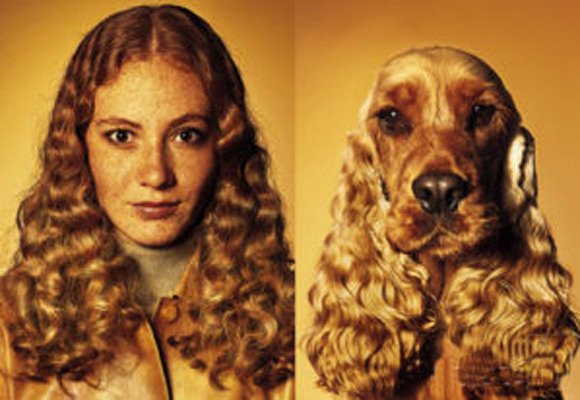
\includegraphics[width=0.9\textwidth]{dogLookAlike.jpg}
\end{center}
\end{frame}
%-------------------------------------------------------------------------------------------------%
\begin{frame}{Are they similar?}
\begin{center}
	
\includegraphics[width=0.9\textwidth]{snoopDog.jpg}
\end{center}
\end{frame}
%-------------------------------------------------------------------------------------------------%
\begin{frame}{What are we after?}
\begin{description}[Motivation:]
	\item[Motivation:]  How is the data structured? Any outliers? 
	\item[Goals:]		\textit{High} intra-cluster similarity and \textit{low} inter-cluster similarity 
\end{description}
\begin{center}
	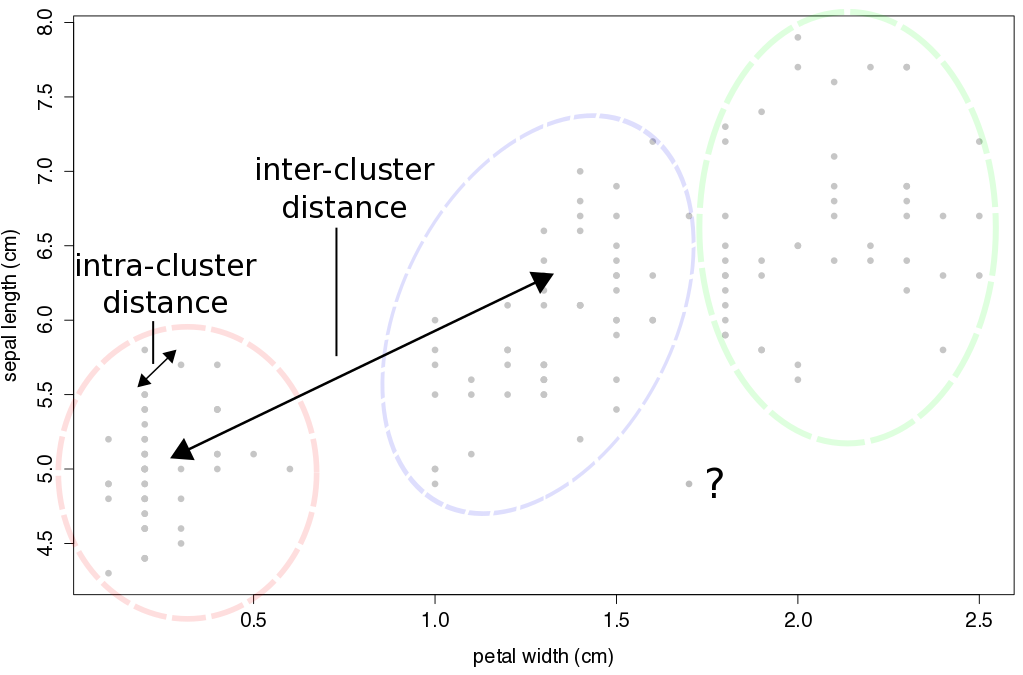
\includegraphics[width=0.9\textwidth]{samplePlot.png}
\end{center}
% Mention that it's a good example of limitation of statistics when analysing this data coz n<<p
\end{frame}

%-------------------------------------------------------------------------------------------------%
\begin{frame}{Major types of clustering methods}
\small
\begin{columns}
\column{0.6\textwidth}
\begin{description}[Distribution-based:]\addtolength{\itemsep}{3\baselineskip}
	\item<2-> [Partitional:] The data (feature) space is partitioned into $k$ regions
	\item<3-> [Hierarchical:] Iteratively merging small clusters into larger ones (\textit{agglomerative})
	or breaking large clusters into smaller ones (\textit{divisive})
	\item<4-> [Distribution-based:] Fit $k$ multivariate statistical distributions 
\end{description}
\column{0.4\textwidth}	
\begin{center}
	\visible<2->{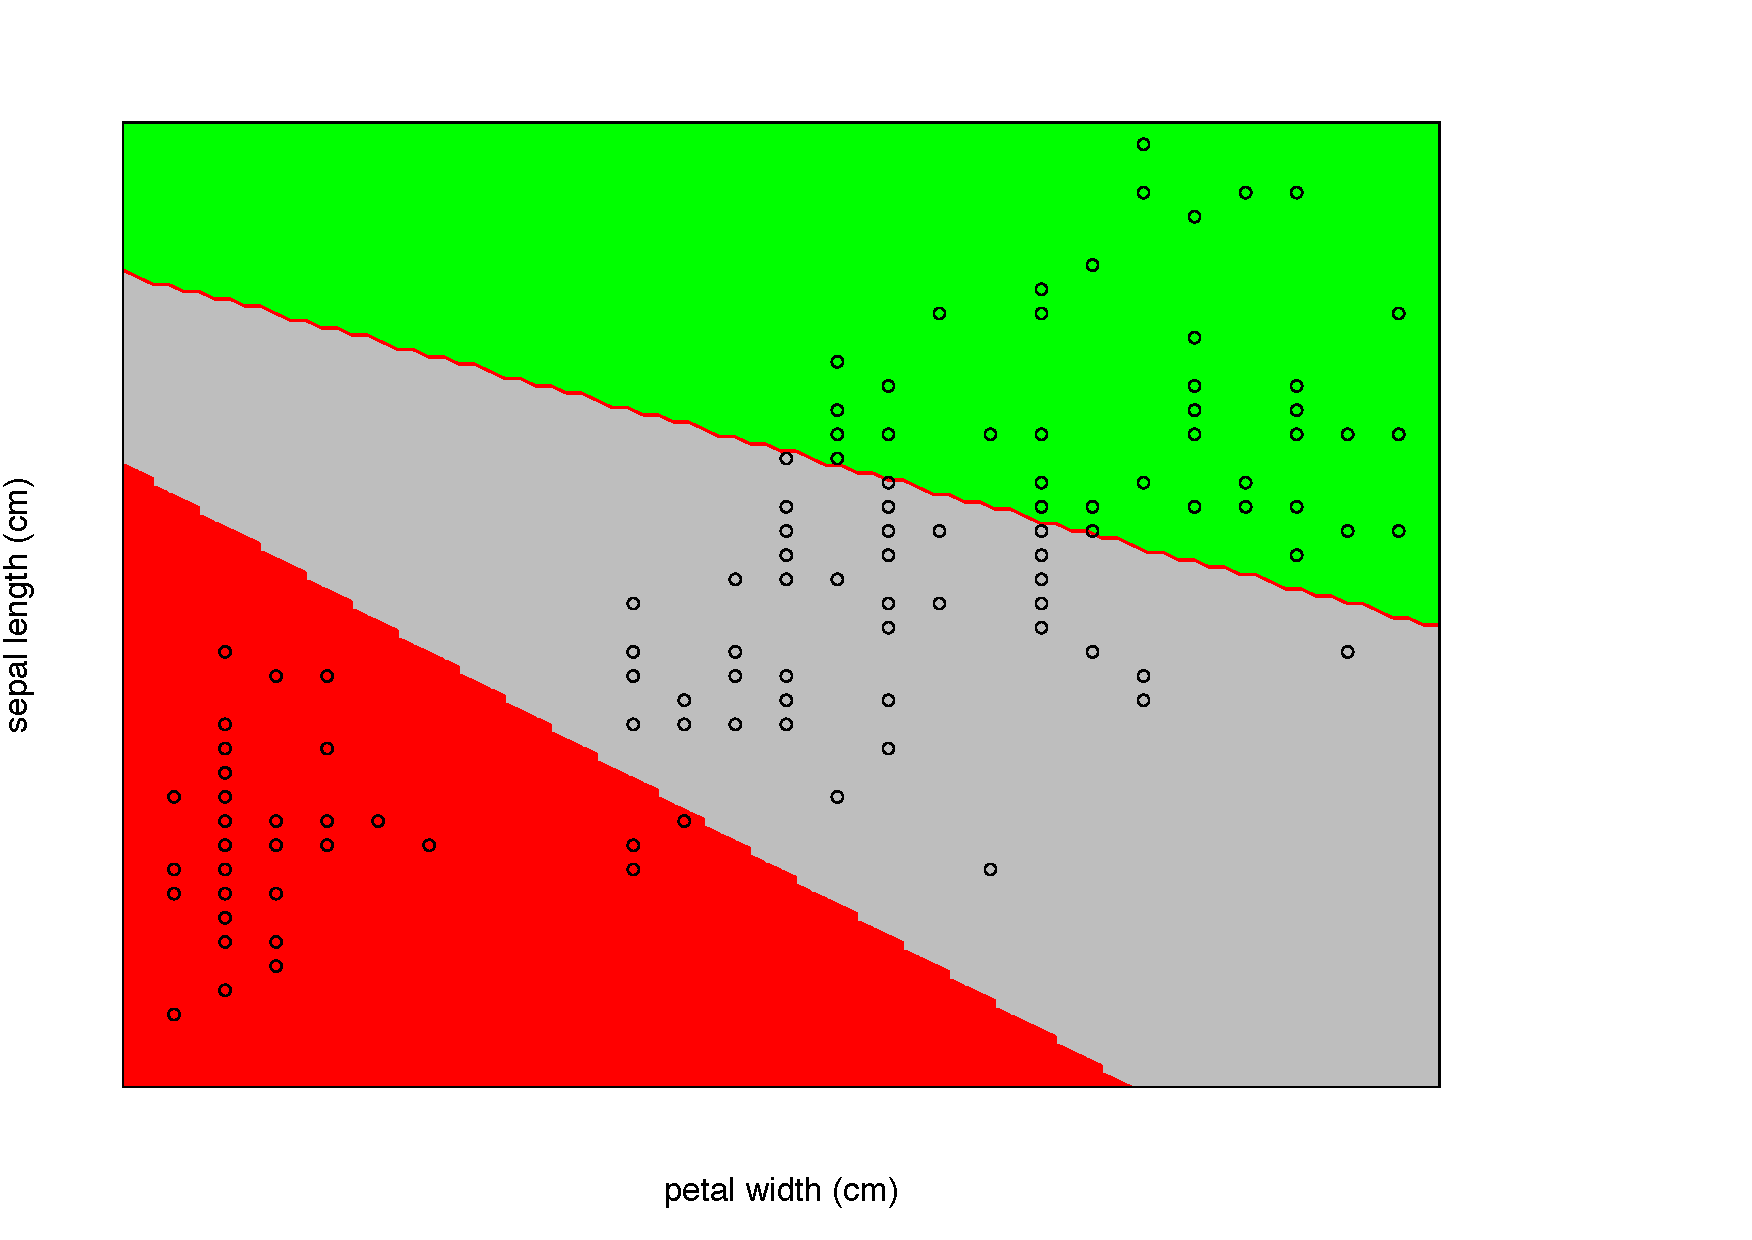
\includegraphics[width=0.68\textwidth]{partitional.pdf}}
	\vfill
	\visible<3->{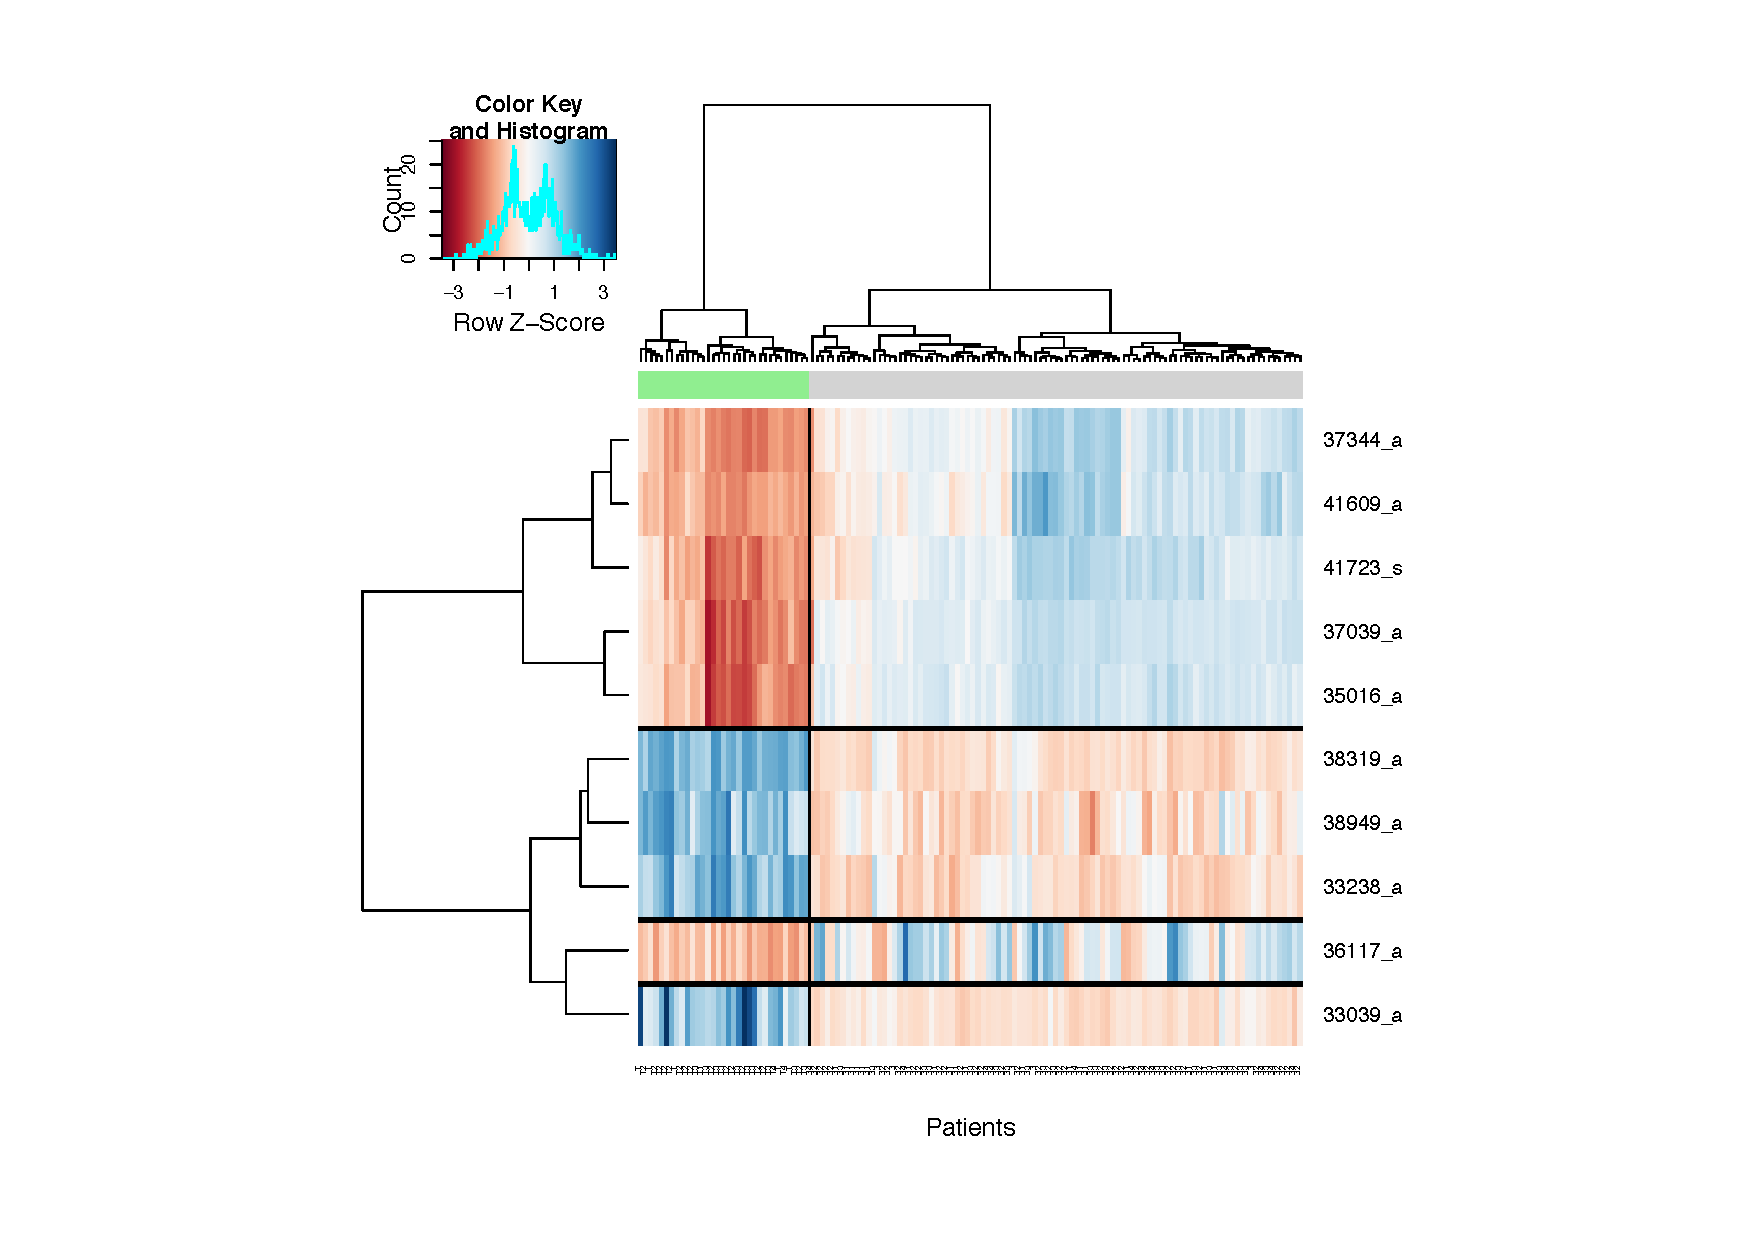
\includegraphics[width=0.68\textwidth]{geneExpression.pdf}}
	\vfill
	\visible<4->{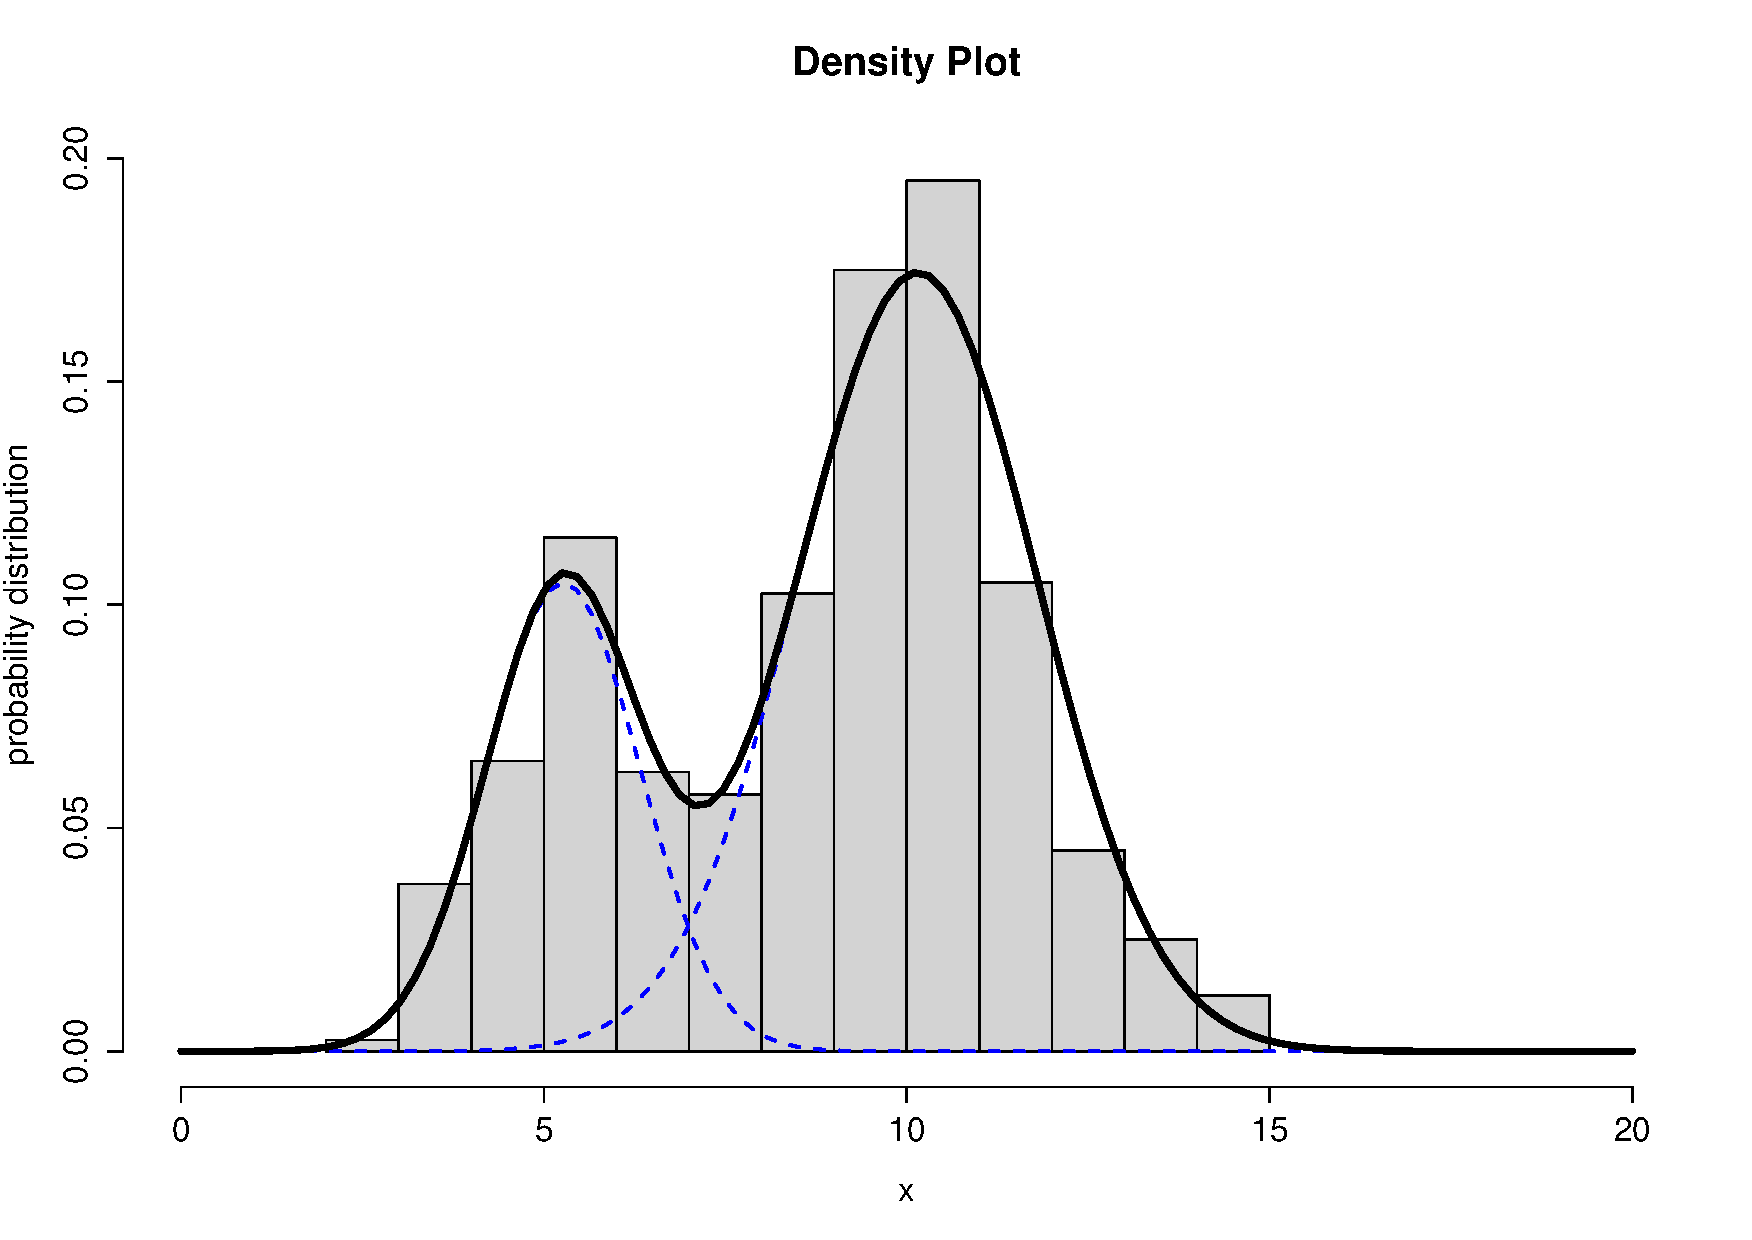
\includegraphics[width=0.68\textwidth]{gmm1D.pdf}}
\end{center}
\end{columns}
\end{frame}
\normalsize
%-------------------------------------------------------------------------------------------------%
\begin{frame}{Similarity measures}
\begin{itemize}\addtolength{\itemsep}{0.5\baselineskip}
	\item A \textit{distance} metric quantifies how \textit{close} two data points are
	\item Several ways to define this distance which has a direct impact on the clustering result
\end{itemize}
\vfill
\begin{center}
	\visible<1->{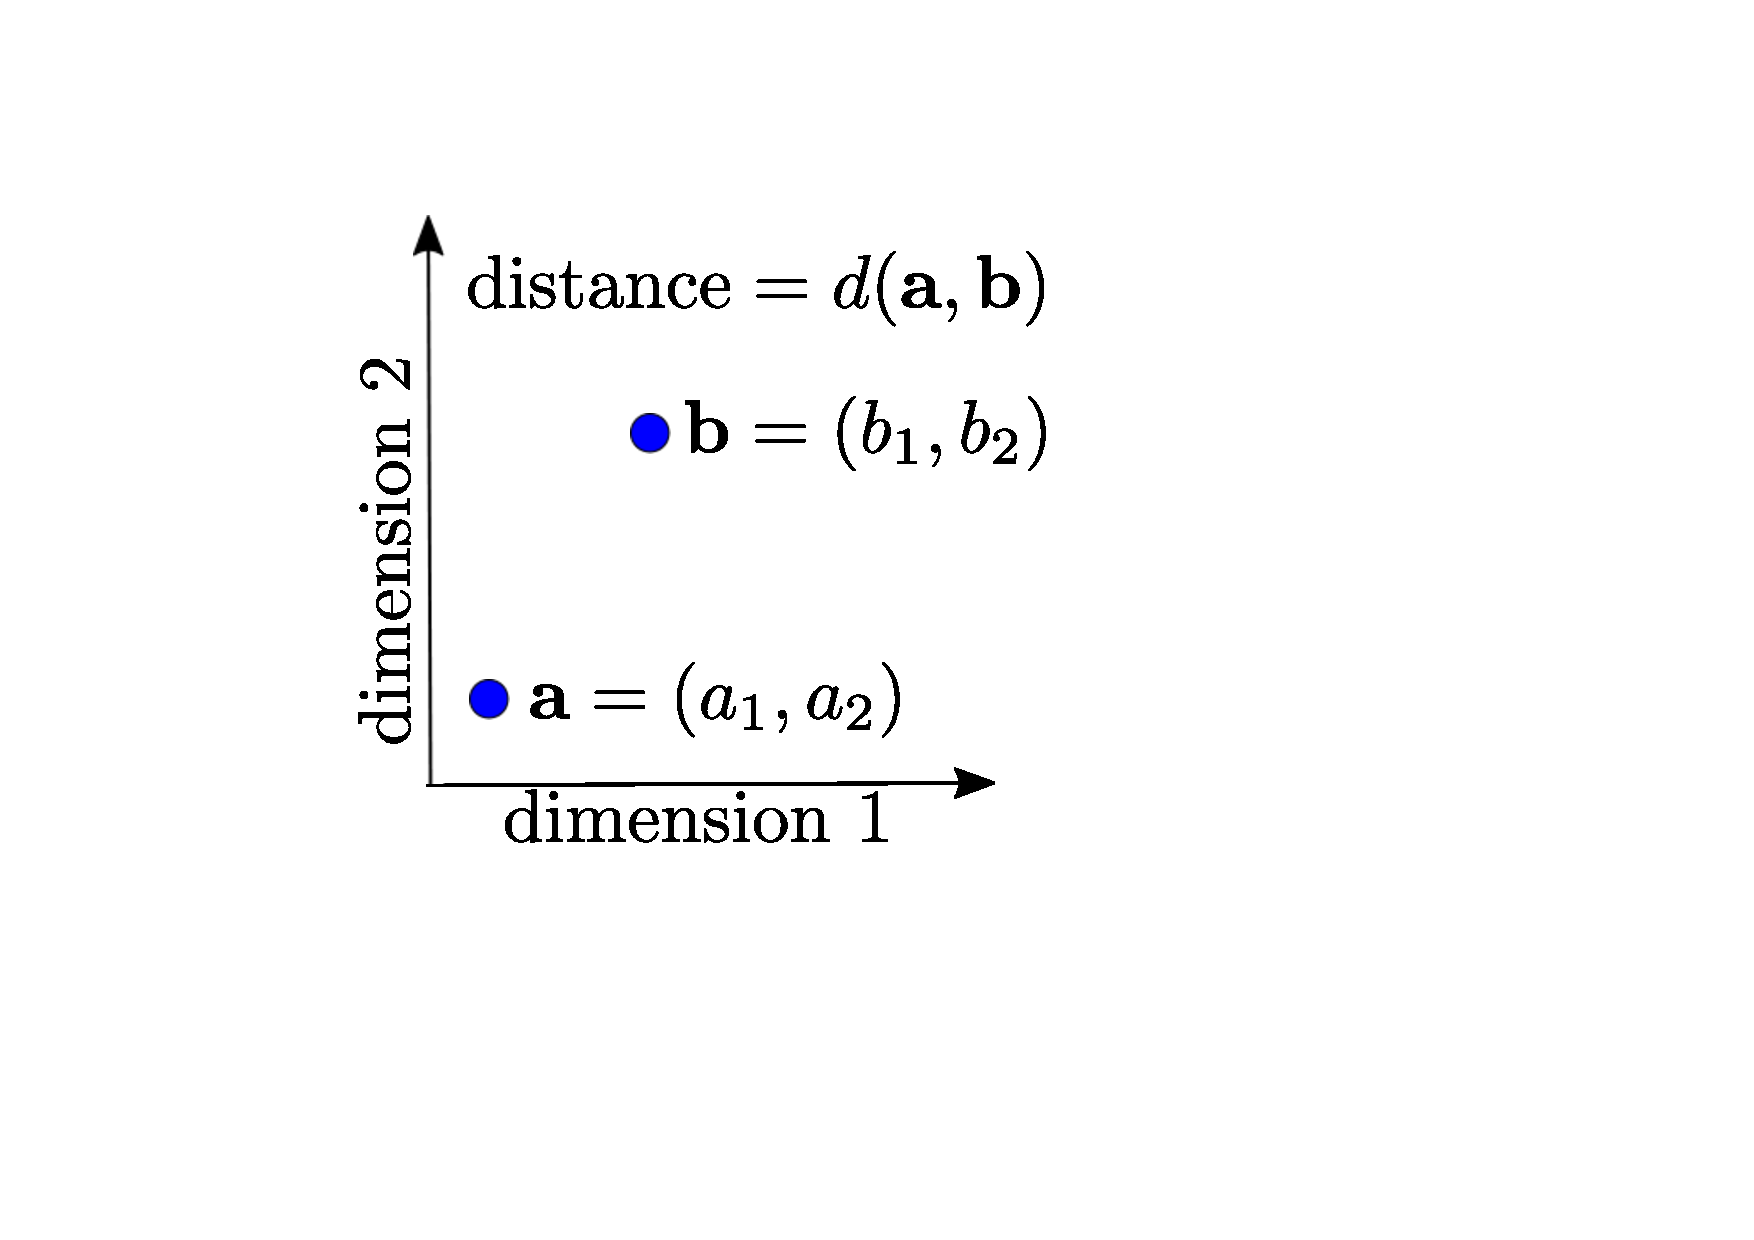
\includegraphics[width=0.4\textwidth]{distance.pdf}}
	\visible<2->{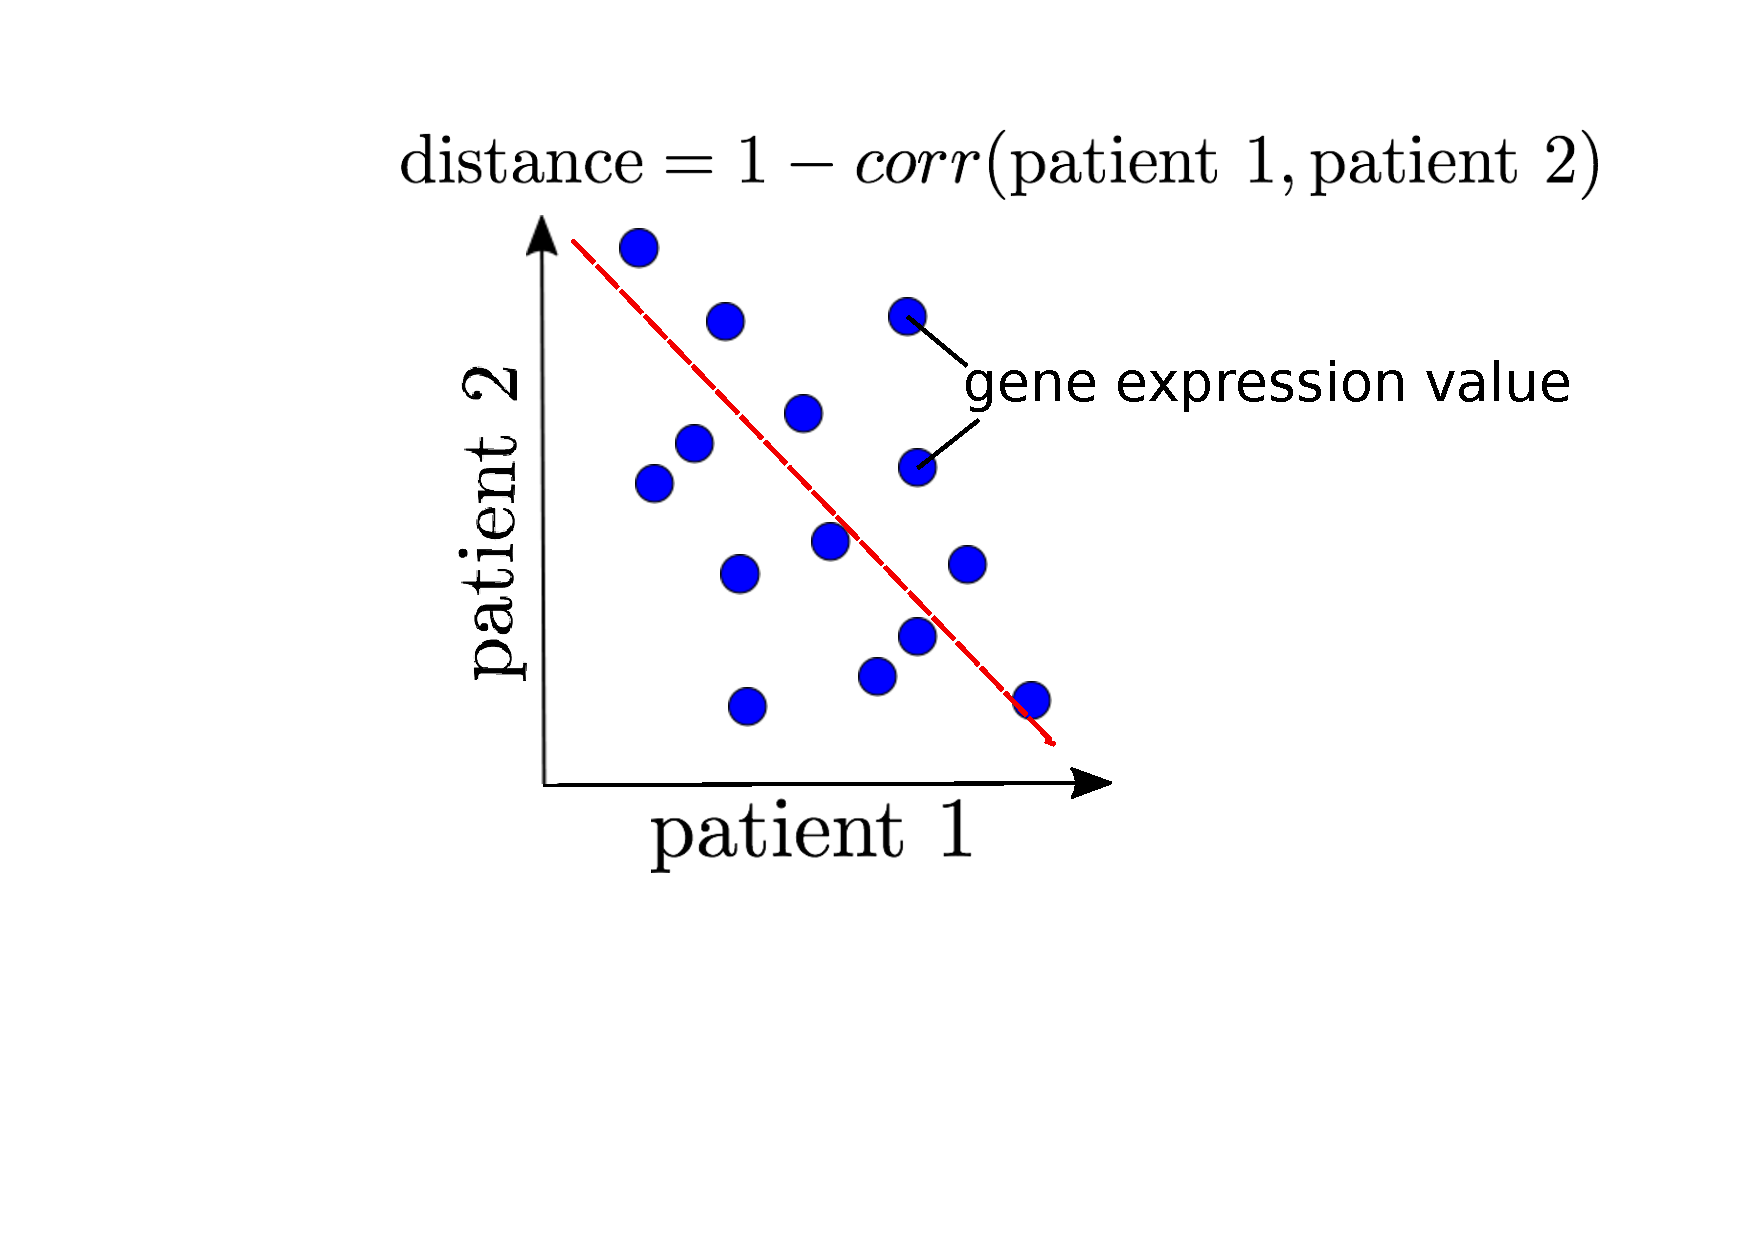
\includegraphics[width=0.59\textwidth]{corrDistance.pdf}}
\end{center}
\end{frame}
% Note: We can also take 1-abs(corr) to consider anti-correlations as being similar
% %-------------------------------------------------------------------------------------------------%
% \begin{frame}{Similarity measures}
% \vspace{-1cm}
% \begin{columns}
% \column{0.68\textwidth}
% What is the distance $d(\mathbf{a,\ b})$ between $\mathbf{a}$ and $\mathbf{b}$?
% \column{0.32\textwidth}
% \begin{center}
% 	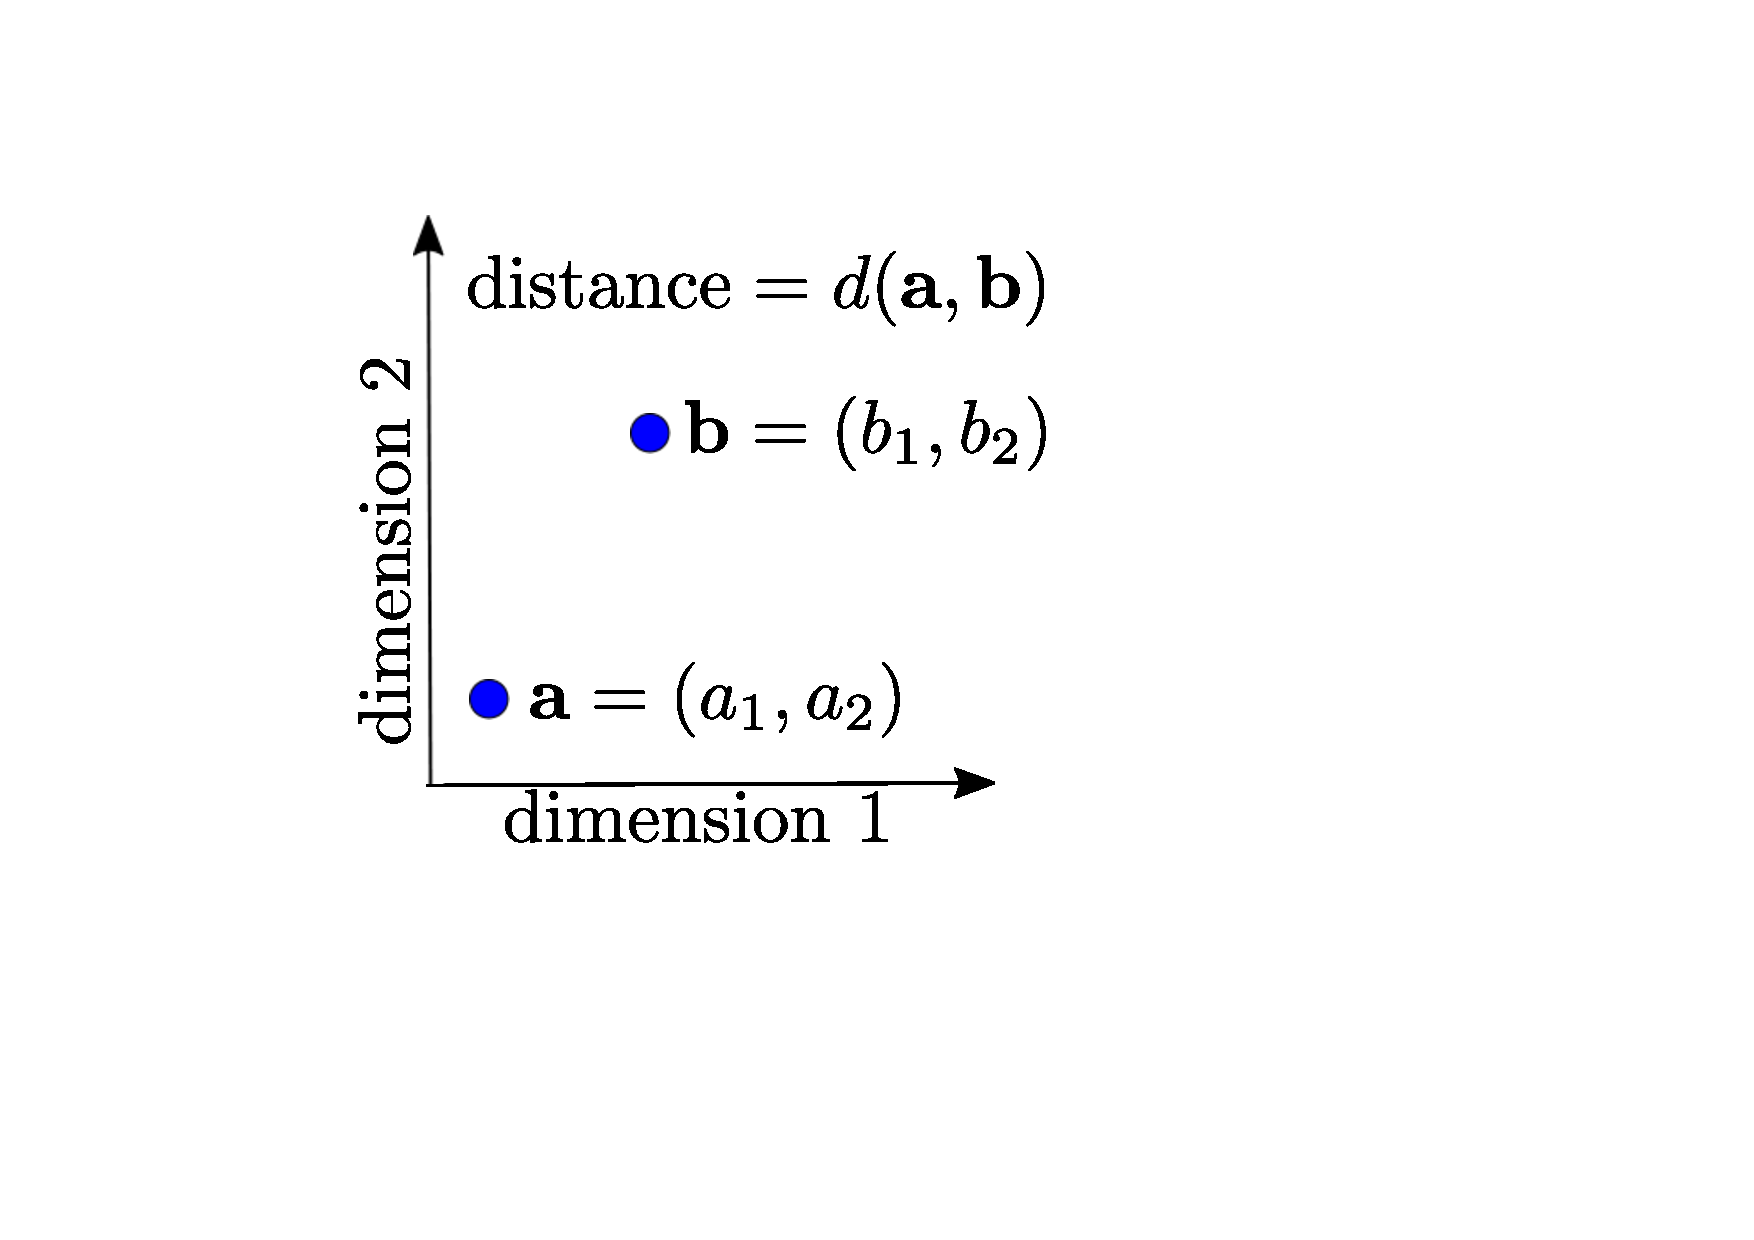
\includegraphics[width=\textwidth]{distance.pdf}
% \end{center}
% \end{columns}
% \begin{columns}
% \column{0.44\textwidth}
% \visible<2->{\begin{block}{example: $\mathbf{a,\ b}\in \mathbb{R}^2$}
% \begin{itemize}\addtolength{\itemsep}{1\baselineskip}
% 	\item<2-> \textbf{Manhattan} 
% 	$\vert a_1 - b_1 \vert + \vert a_2 - b_2 \vert$
% 	\item<3-> \textbf{Euclidean} 
% 	$\sqrt{(a_1 - b_1)^2 + (a_2 - b_2)^2}$
% 	\item<4-> \textbf{Minkowski (p-norm)} 
% 	$\sqrt[p]{\vert a_1 - b_1 \vert^p + \vert a_2 - b_2 \vert^p}$
% \end{itemize}
% \end{block}}
% \column{0.55\textwidth}	
% \visible<2->{\begin{block}{in general: $\mathbf{a,\ b}\in \mathbb{R}^d$}
% \begin{itemize}\addtolength{\itemsep}{1.6\baselineskip}
% 	\item[]<2->
% 	$\sum_{i=1}^{d}\vert a_i - b_i \vert = \Vert \mathbf{a} - \mathbf{b} \Vert_1$
% 	\item[]<3->
% 	$\left(\sum_{i=1}^{d}(a_i - b_i)^2\right)^{\frac{1}{2}} = \Vert \mathbf{a} - \mathbf{b} \Vert_2$
% 	\item[]<4->
% 	$\left(\sum_{i=1}^{d}\vert a_i - b_i \vert^p\right)^{\frac{1}{p}} = \Vert \mathbf{a} - \mathbf{b} \Vert_p$
% \end{itemize}
% \end{block}}
% \end{columns}
% \end{frame}
% %-------------------------------------------------------------------------------------------------%
% \begin{frame}{Similarity measures}
% \vspace{-1cm}
% \begin{columns}
% \column{0.68\textwidth}
% What is the distance $d(\mathbf{a,\ b})$ between $\mathbf{a}$ and $\mathbf{b}$?
% \column{0.32\textwidth}
% \begin{center}
% 	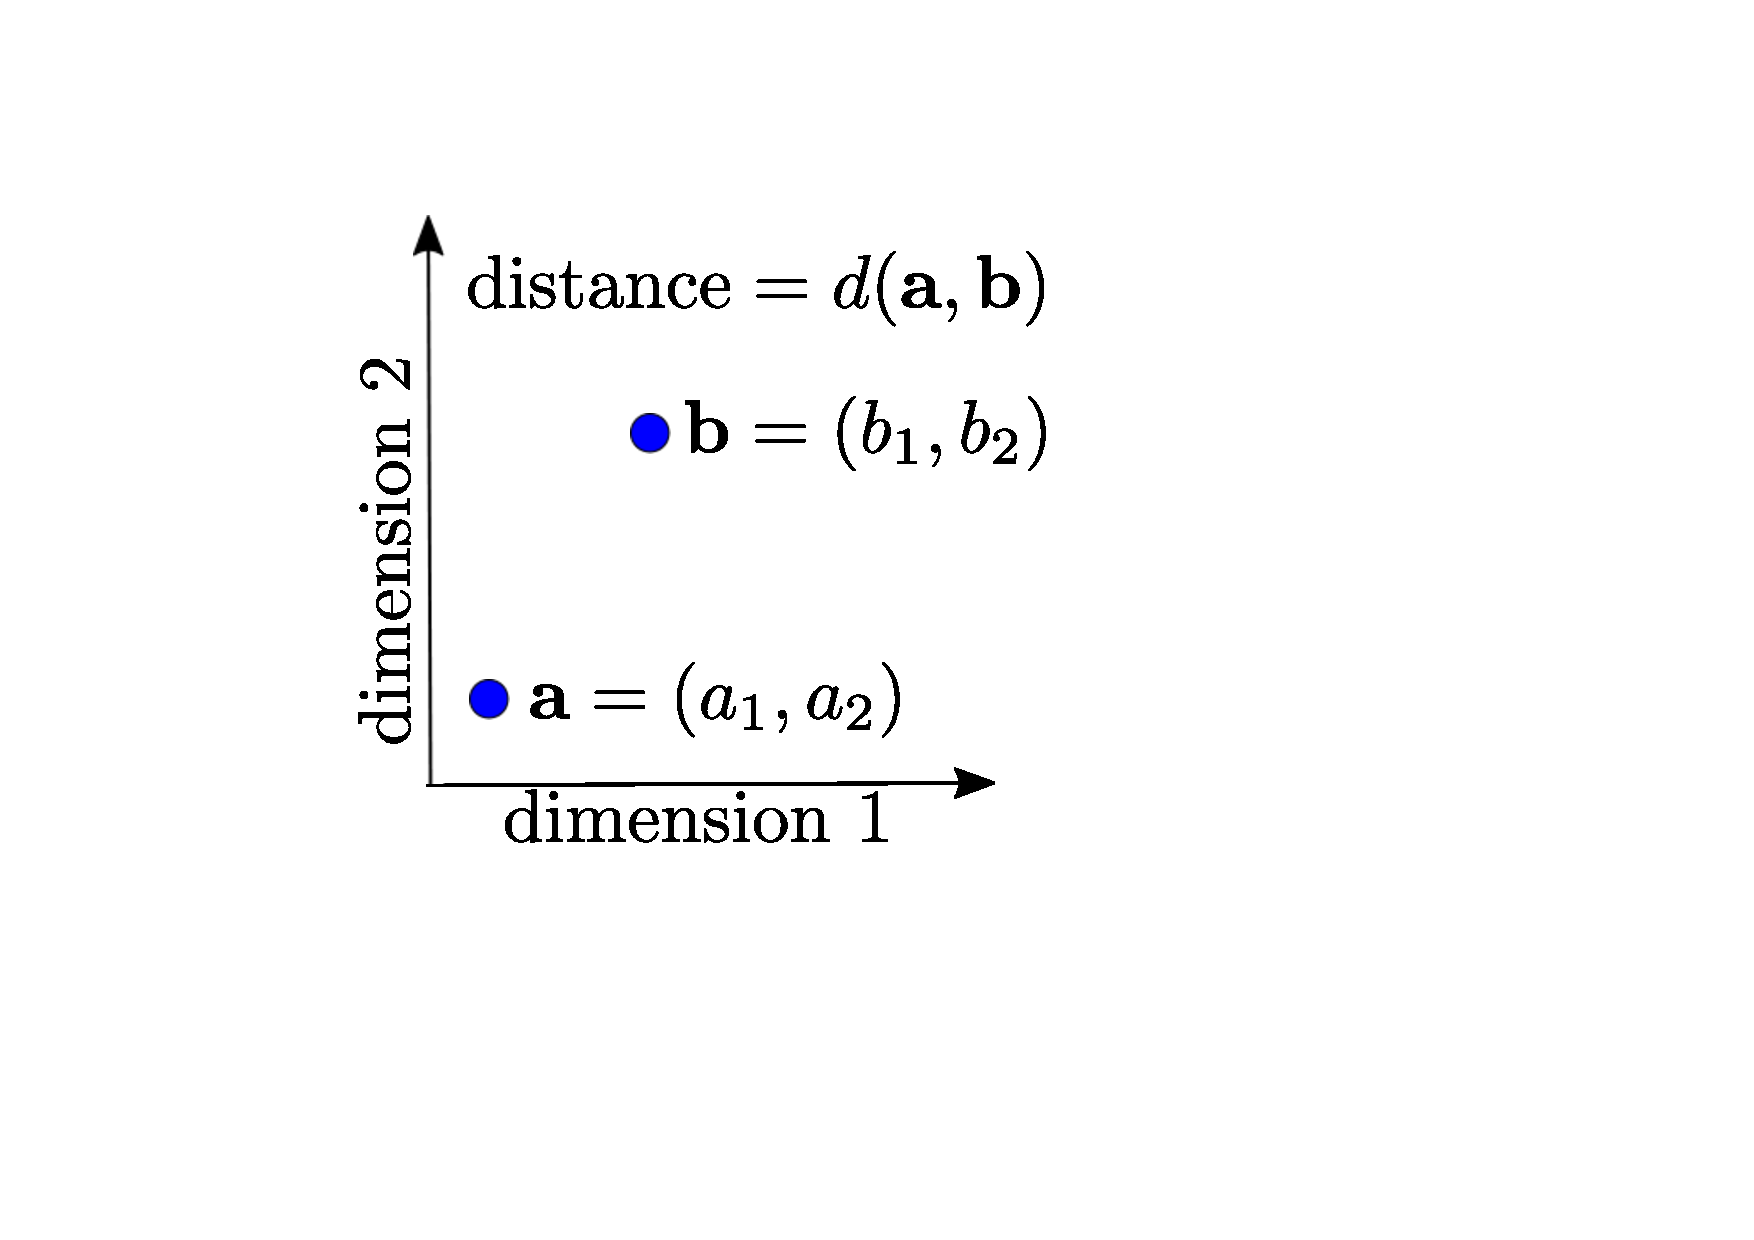
\includegraphics[width=\textwidth]{distance.pdf}
% \end{center}
% \end{columns}
% \begin{columns}
% \column{0.44\textwidth}
% \begin{block}{example: $\mathbf{a,\ b}\in \mathbb{R}^2$}
% \begin{itemize}\addtolength{\itemsep}{1.46\baselineskip}
% 	\item<2-> \textbf{Canberra} 
% 	$\frac{\vert a_1 - b_1 \vert}{\vert a_1 \vert + \vert b_1 \vert} + \frac{\vert a_2 - b_2 \vert}{\vert a_2 \vert + \vert b_2 \vert} $
% 	\item<3-> \textbf{Cosine similarity} 
% 	$\frac{a_1b_1 + a_2b_2}{\sqrt{a_1^2 + a_2^2}\sqrt{b_1^2 + b_2^2}}$
% 	\item<4-> \textbf{Correlation distance}
% \end{itemize}
% \end{block}
% \column{0.55\textwidth}	
% \begin{block}{in general: $\mathbf{a,\ b}\in \mathbb{R}^d$}
% \begin{itemize}\addtolength{\itemsep}{1.85\baselineskip}
% 	\item[]<2->
% 	$\sum_{i=1}^{d}\frac{\vert a_i - b_i \vert}{\vert a_i \vert + \vert b_i \vert}$
% 	\item[]<3->
% 	$\frac{\sum_{i=1}^{d}a_ib_i}{\sqrt{\sum_{i=1}^{d}(a_i)^2}\sqrt{\sum_{i=1}^{d}(b_i)^2}} = \frac{\mathbf{a.b}}{\Vert a \Vert_2 \Vert b \Vert_2}$
% 	\item[]<4->
% 	Pearson ($\rho$), Spearman, Kendall ($\tau$)
% \end{itemize}
% \end{block}
% \end{columns}
% \end{frame}
%-------------------------------------------------------------------------------------------------%
\begin{frame}[fragile]
\frametitle{$k$-means clustering}
\begin{lstlisting}[style=RCode]
fit <- kmeans(x, centers)
# x - numeric matrix of data
# centers - no. of clusters k 
\end{lstlisting}
\begin{enumerate}\addtolength{\itemsep}{0.5\baselineskip}
	\item<2-> Select $k$ centroids at random
	\item<3-> Calculate distance between centroids and each data point 
	\item<4-> Assign each data point to the closest centroid
	\item<5-> Compute new centroids; the average of all data points in that cluster
	\item<6-> Repeat steps 2 to 4 until data points remain in the same cluster or some maximum number of iterations reached
\end{enumerate}
\vfill
\visible<7->{\textbf{Note}: $k$-means clustering should \textit{only} be used with continuous data}
\end{frame}
%-------------------------------------------------------------------------------------------------%
\begin{frame}{$k$-means clustering}
	\begin{center}
		\includegraphics<1>[width=0.68\textwidth]{iteration1.pdf}
		\includegraphics<2>[width=0.68\textwidth]{iteration2.pdf}
		\includegraphics<3>[width=0.68\textwidth]{iteration3.pdf}
		\includegraphics<4>[width=0.68\textwidth]{iteration4.pdf}
		\includegraphics<5>[width=0.68\textwidth]{iteration5.pdf}
		\includegraphics<6>[width=0.68\textwidth]{iteration6.pdf}
		\includegraphics<7>[width=0.68\textwidth]{iteration7.pdf}
	\end{center}
\end{frame}
%-------------------------------------------------------------------------------------------------%
\begin{frame}{$k$-means clustering}
\begin{exampleblock}{Pros}
\begin{itemize}
	\item Simple and intuitive
	\item Computationally inexpensive/fast 
\end{itemize}
\end{exampleblock}
\vfill
\begin{alertblock}{Cons}
\begin{itemize}
	\item What is $k$?
	\item Only applicable to continuous data where a mean is defined
	\item No guarantee of a global optimum solution
\end{itemize}
\end{alertblock}
\end{frame}
%-------------------------------------------------------------------------------------------------%
\begin{frame}[fragile]
\frametitle{Agglomerative hierarchical clustering}
\begin{lstlisting}[style=RCode]
d <- dist(as.matrix(data), method)
# data - data frame 
# method - distance method e.g "euclidean" or "manhattan"
fit <- hclust(d, method) 
# method - linkage function e.g "complete" or "single"
\end{lstlisting}
\begin{enumerate}\addtolength{\itemsep}{0.5\baselineskip}
	\item<2-> Assign each data point as its own cluster
	\item<3-> Compute distance between each cluster
	\item<4-> Merge the closest pair into a single cluster
	\item<5-> Repeat 2 to 3 until you're left with one cluster
\end{enumerate}
\vfill
\visible<6->{\textbf{Note}: Step 3 is \textit{key}, the distance method and linkage function dictate the final result}
\end{frame}
%-------------------------------------------------------------------------------------------------%
\begin{frame}{Hierarchical clustering: Link method}
How do we compute the inter-cluster distance? The \textit{linkage function}
\begin{columns}
\column{0.6\textwidth}
\begin{description}[Complete:]\addtolength{\itemsep}{0.8\baselineskip}
	\item<2-> [Centroid:] mean of data points (same as in $k$-means)
	\item<3-> [Single:] distance between closest pair of points
	\item<4-> [Complete:] distance between furthest pair of points
	\item<5-> [Average:] mean pairwise distance between all points
\end{description}
\column{0.4\textwidth}	
\begin{center}
	\visible<2->{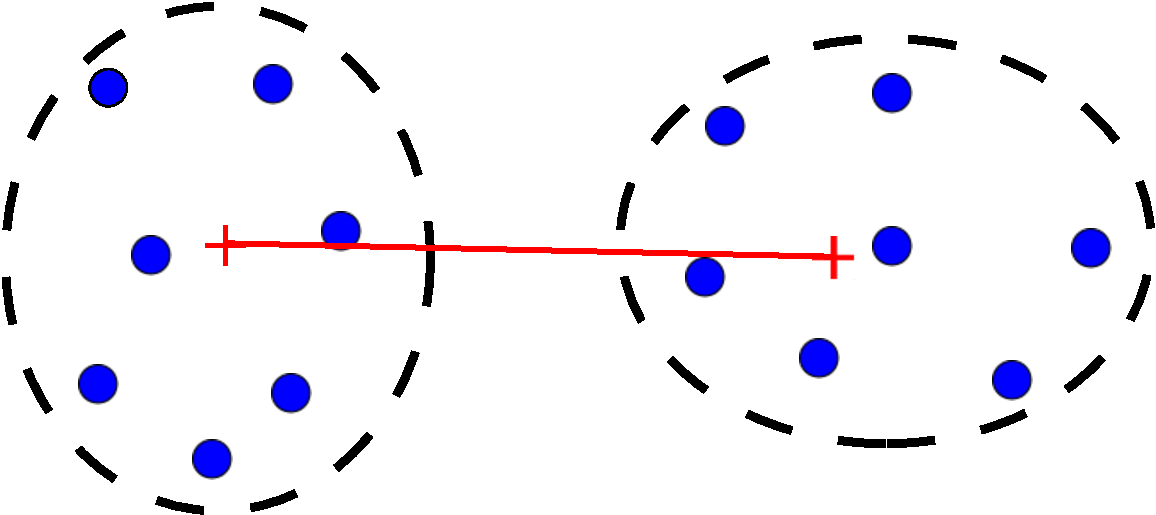
\includegraphics[width=0.75\textwidth]{centroid.pdf}}
	\vfill
	\visible<3->{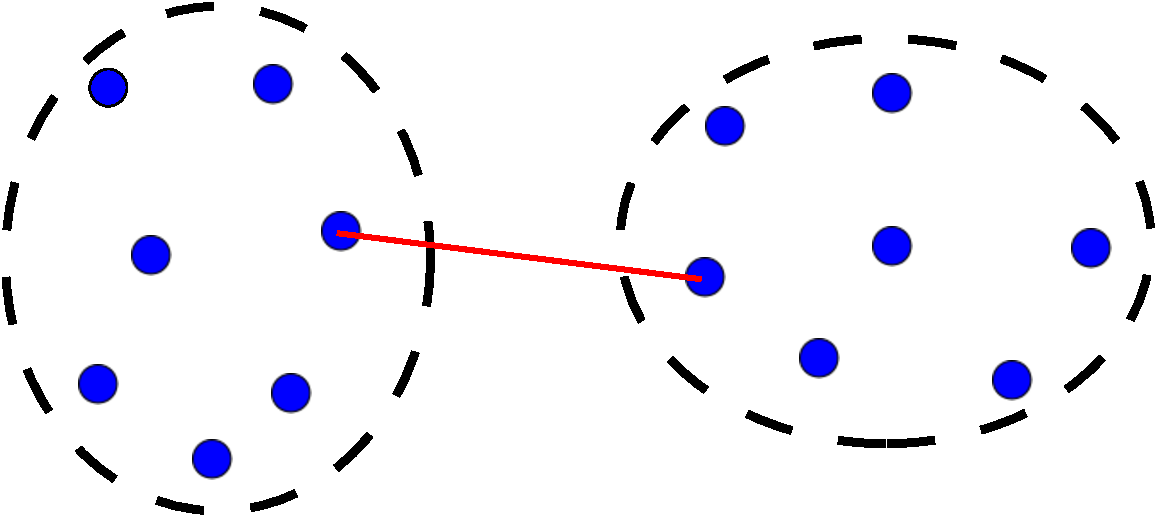
\includegraphics[width=0.75\textwidth]{single.pdf}}
	\vfill
	\visible<4->{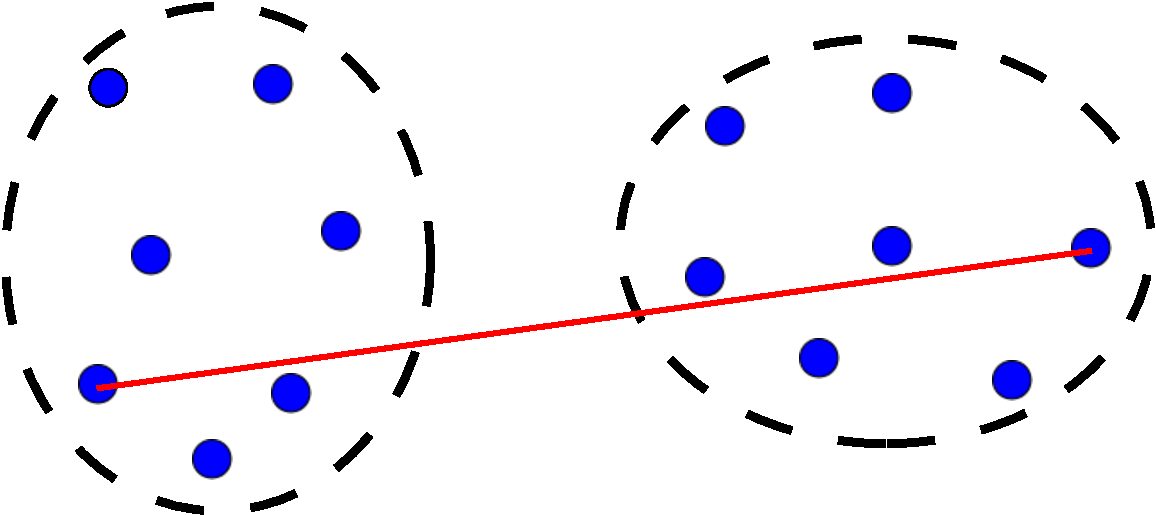
\includegraphics[width=0.75\textwidth]{complete.pdf}}
	\vfill
	\visible<5->{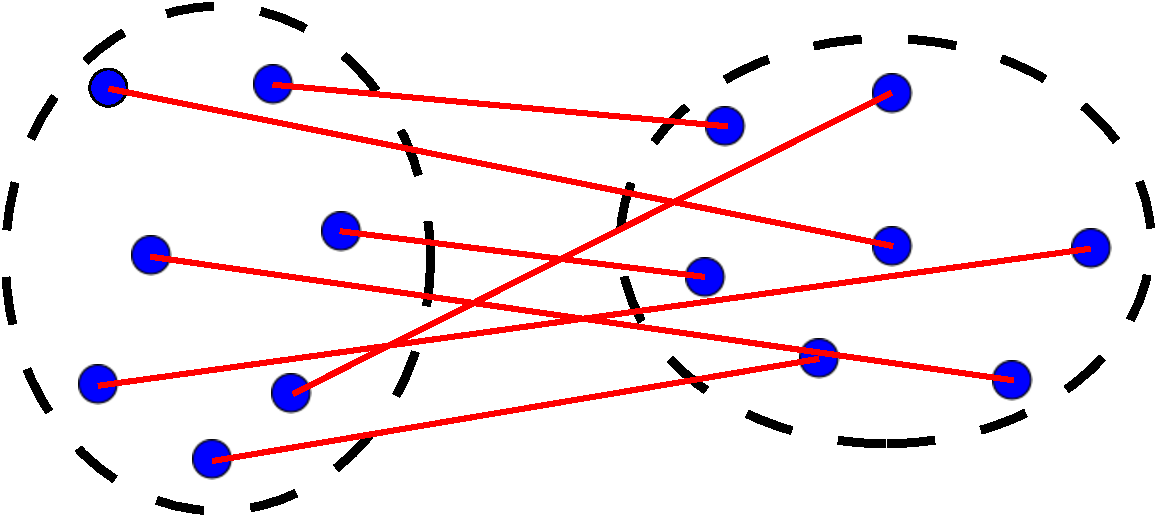
\includegraphics[width=0.75\textwidth]{average.pdf}}
\end{center}
\end{columns}
\end{frame}
%-------------------------------------------------------------------------------------------------%
\begin{frame}{Hierarchical clustering in gene expression studies}
\begin{center}
	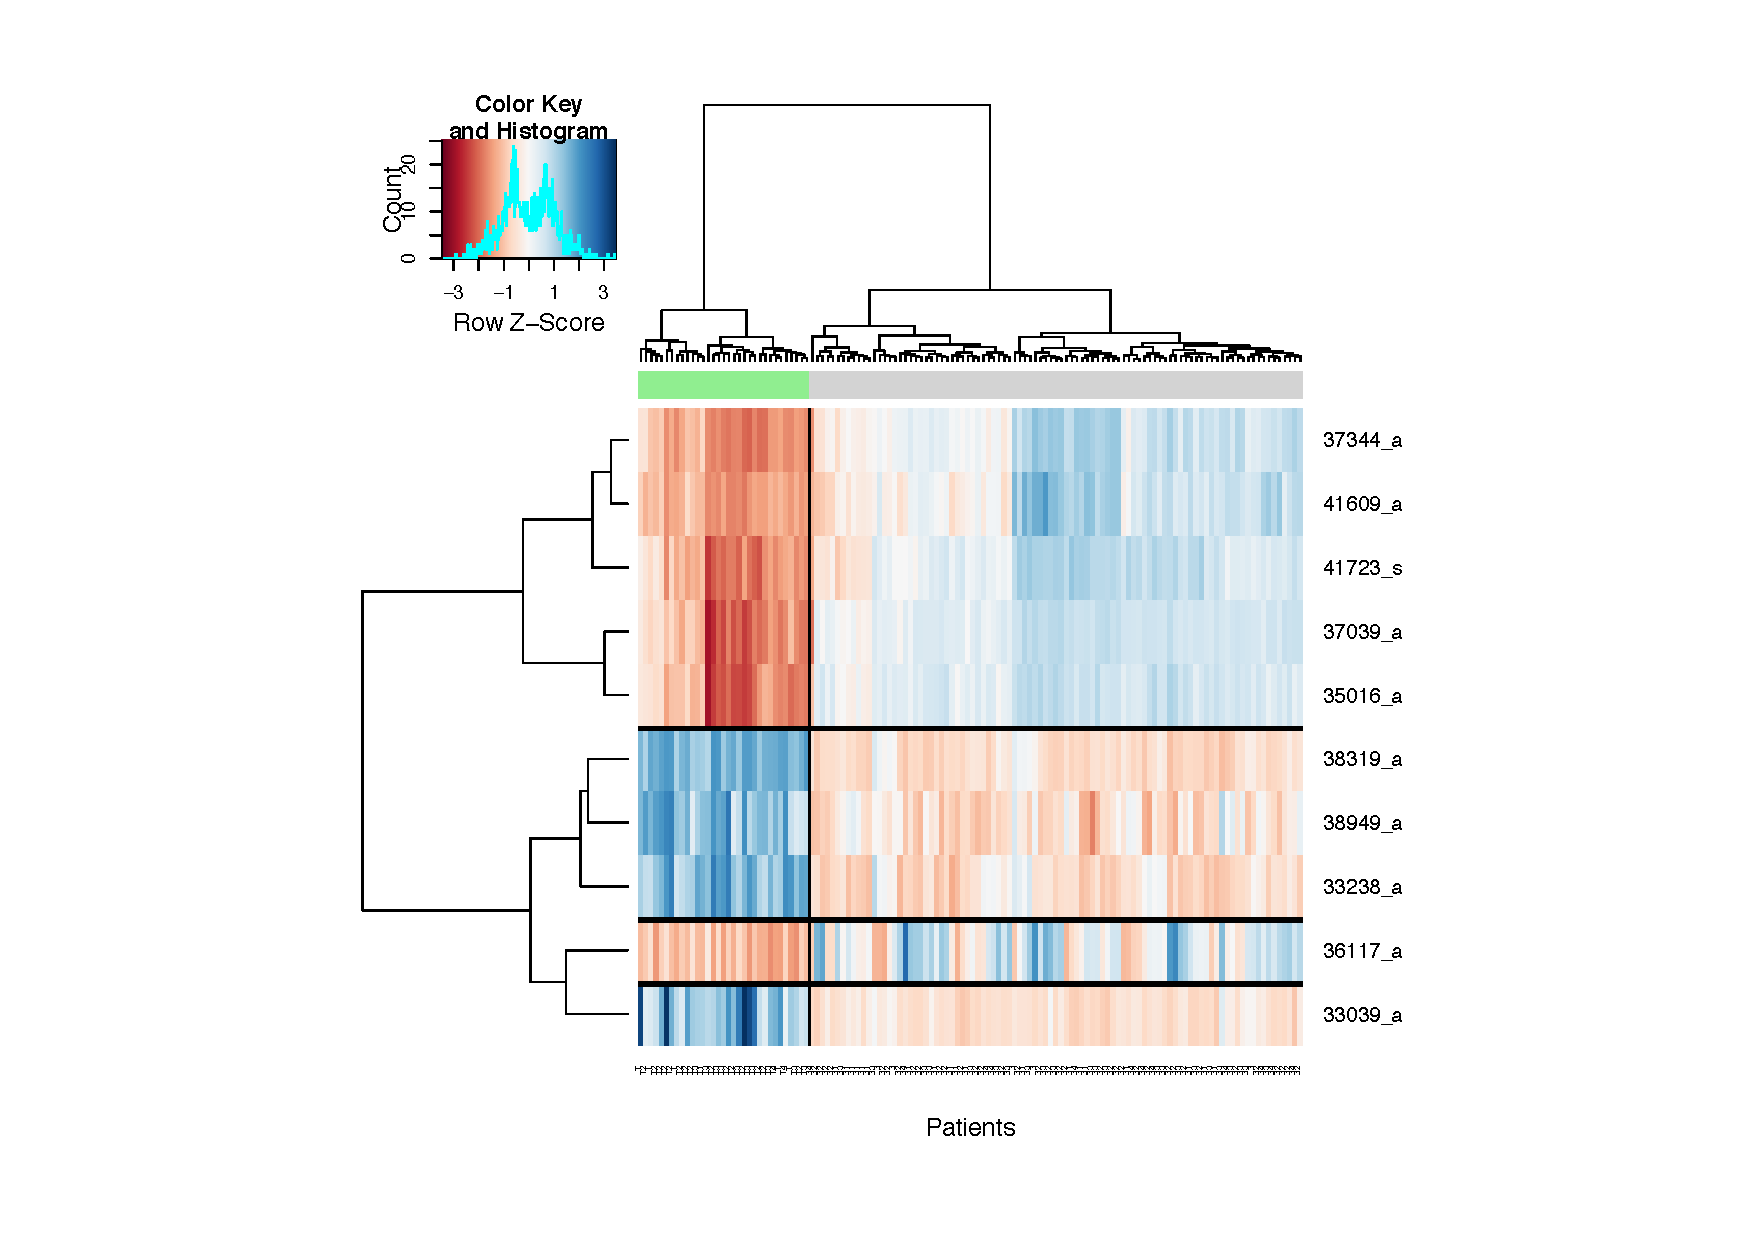
\includegraphics[width=0.67\textwidth]{geneExpression.pdf}
\end{center}
\end{frame}
%-------------------------------------------------------------------------------------------------%
\begin{frame}{Hierarchical clustering}
\begin{exampleblock}{Pros}
\begin{itemize}
	\item No need to specify $k$
	\item Results can be visualised nicely irrespective of number of dimensions 
\end{itemize}
\end{exampleblock}
\vfill
\begin{alertblock}{Cons}
\begin{itemize}
	\item Can be computationally expensive
	\item Interpretation is subjective. Where should we draw the line (to separate clusters)?
	\item Choice of distance method and linkage function can significantly change the result 
\end{itemize}
\end{alertblock}
\end{frame}
%-------------------------------------------------------------------------------------------------%
\begin{frame}[fragile]
\frametitle{Gaussian mixture models}
\begin{lstlisting}[style=RCode]
library(mclust)
fit <- Mclust(data, G)
# data - data frame 
# G - no. of Gaussians
\end{lstlisting}
\begin{enumerate}
	\item Fit $k$ multivariate Gaussian distributions
\end{enumerate}
\vfill
The Expectation-Maximisation (EM) algorithm is used to estimate the parameters $\pi_i$ (mixing coefficients), $\mu_i$ and $\sigma_i$
$$
p(x) = \sum_{i=1}^k \pi_i \mathcal{N}(x|\mu_i, \Sigma_i)\ \mathrm{and}\ \sum_{i=1}^k \pi_i = 1
$$
Can be seen as a ``soft'' version of $k$-means because \textit{every} point is part of \textit{every} cluster but
with varying levels of membership
\end{frame}
%-------------------------------------------------------------------------------------------------%
\begin{frame}{Gaussian mixture models}
\begin{center}
	\includegraphics<1>[width=0.95\textwidth]{gmm1D.pdf}
	\includegraphics<2>[width=0.95\textwidth]{gmm2D.pdf}
\end{center}
\end{frame}
%-------------------------------------------------------------------------------------------------%
\begin{frame}{Gaussian mixture models}
\begin{exampleblock}{Pros}
\begin{itemize}
	\item Intuitive interpretation
	\item Computationally inexpensive
\end{itemize}
\end{exampleblock}
\vfill
\begin{alertblock}{Cons}
\begin{itemize}
	\item What is $k$?
	\item Strong assumption on the data (normality)
	\item No guarantee of a global optimum solution
\end{itemize}
\end{alertblock}
\end{frame}
%-------------------------------------------------------------------------------------------------%
\begin{frame}{How do we determine the correct number of clusters?}
\textbf{Short answer}: you can't
\vfill
Because data is unlabelled the correct number of $k$ is ambiguous
\vfill
However we can plot some indices as a function of $k$ to help us evaluate cluster validity:
\vfill
\begin{itemize}\addtolength{\itemsep}{0.8\baselineskip}
	\item Within and between clusters sum-of-squares distances
	\item Akaike Information Criterion (AIC) or Bayesian Information Criterion (BIC) when using distribution-based methods
	\item Silhouette plot %$-1 \geq s(i) \leq 1$ where:\\
	% $s(i) = 1$, \textit{i}th datum is appropriately clustered (good)\\
	% $s(i) = 0$, \textit{i}th datum is borderline between two clusters (meh.)\\
	% $s(i) = -1$, \textit{i}th datum should be in neighbouring cluster (bad)
\end{itemize}
\end{frame}
%-------------------------------------------------------------------------------------------------%
\begin{frame}{How do we determine the correct number of clusters?}
\begin{center}
	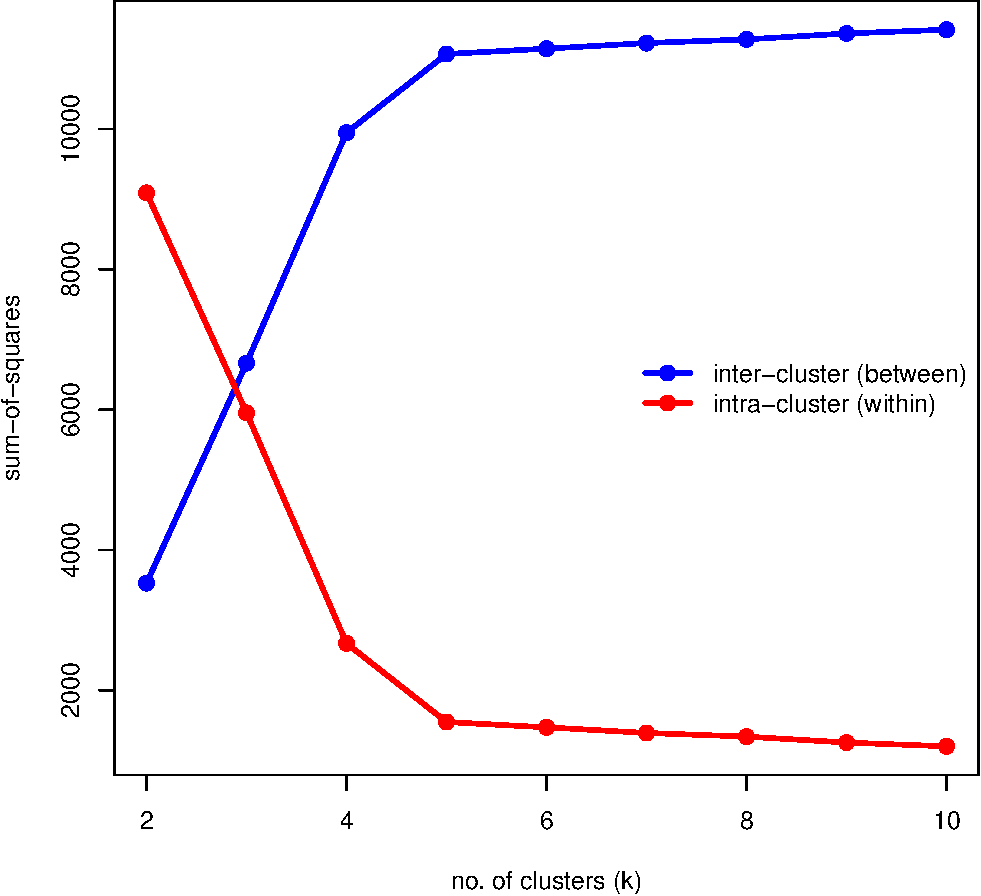
\includegraphics[width=0.48\textwidth]{sumOfSquares.pdf}\hfill	
	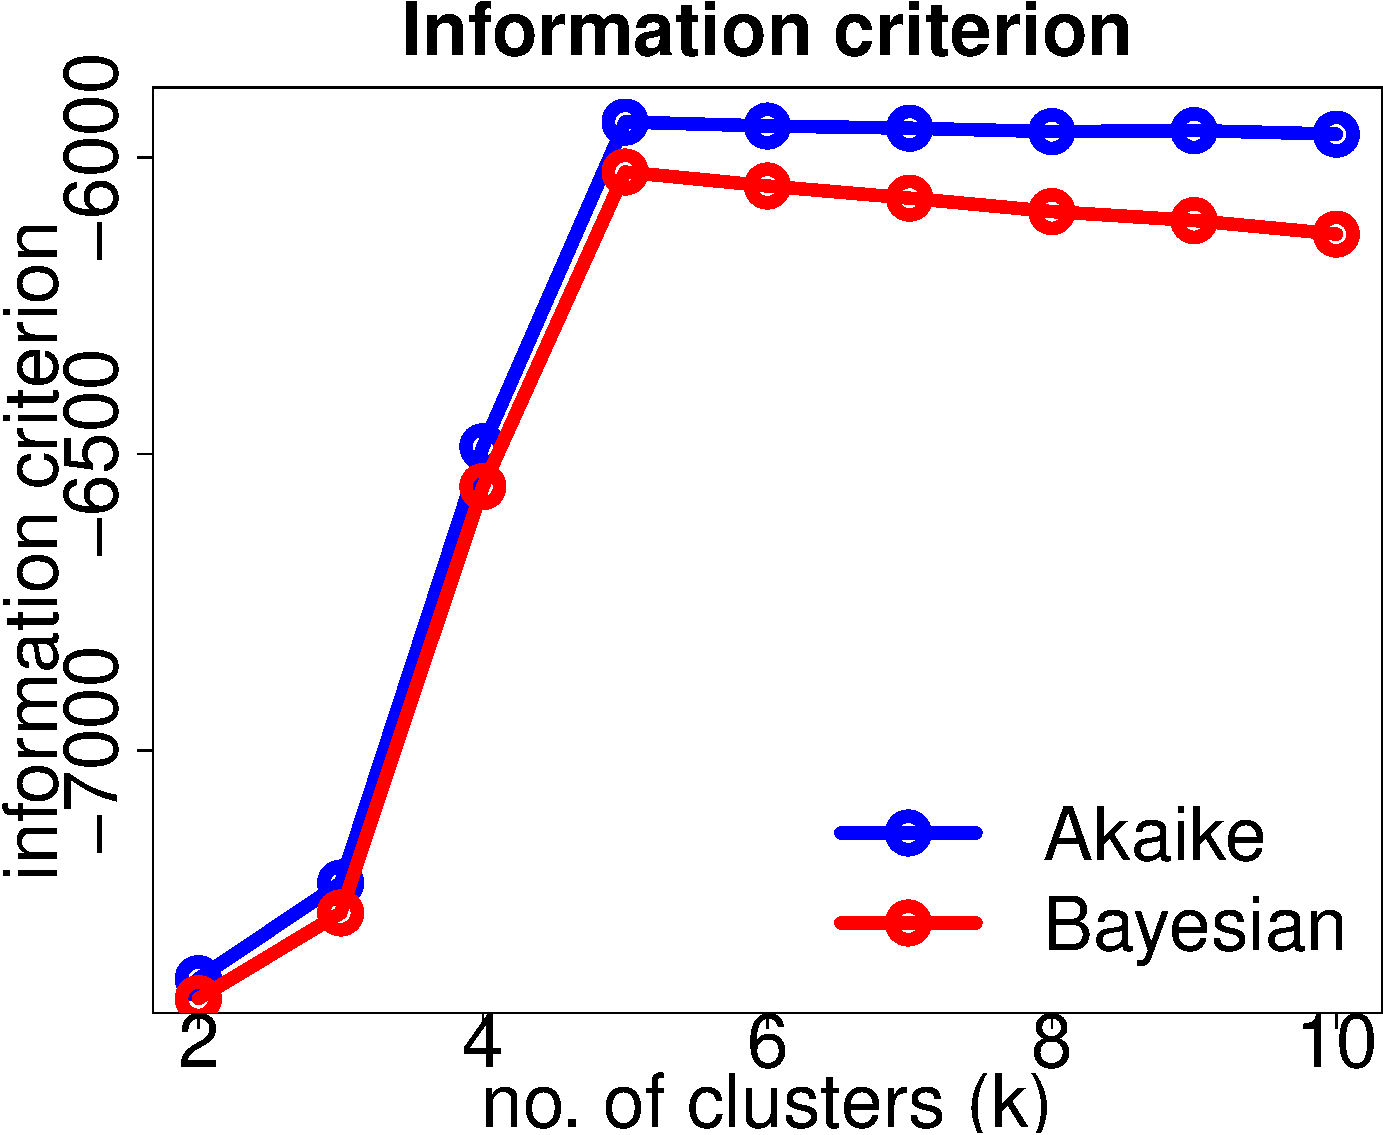
\includegraphics[width=0.48\textwidth]{infoCriterion.pdf}
\end{center}
\end{frame}
% Silhoutte plot result
% 0.71-1.0
% A strong structure has been found

% 0.51-0.70
% A reasonable structure has been found

% 0.26-0.50
% The structure is weak and could be artificial. Try additional methods of data analysis.

% < 0.25
% No substantial structure has been found
%-------------------------------------------------------------------------------------------------%
\begin{frame}[fragile]
\frametitle{How do we determine the correct number of clusters?}
The \textbf{\texttt{NbClust}} package provides 30 different cluster validity metrics. A majority vote can be
taken to deduce the appropriate number of clusters
\vfill
\begin{lstlisting}[style=RCode]
library(NbClust)
NbClust(data, distance, method, min.nc, max.nc, index)
# data - data frame 
# distance - similarity measure e.g "euclidean"
# method - clustering algorithm e.g "kmeans"
# min.nc - min number of clusters to consider
# max.nc - max number of clusters to consider
# index - which indices to compute, "all" computes all of them
\end{lstlisting}
\vspace{-0.5cm}
\textbf{Note}: 
\begin{itemize}\addtolength{\itemsep}{0.3\baselineskip}
	\item Indices \textit{only} give us a ballpark range for ``correct'' number of clusters
	\item {\large \textbf{Are they biologically relevant? Does it make sense?\\Prior knowledge to the rescue}}
	\item E.g how many different phenotypes are you expecting?
\end{itemize}
\end{frame}
%-------------------------------------------------------------------------------------------------%
\end{document}
%-------------------------------------------------------------------------------------------------%
% End of Document
%-------------------------------------------------------------------------------------------------%